\section{Methodology}
\subsection{Description of the data}
The data used by the information system is sourced from three public registers:
\begin{enumerate}
	\item The Central Insolvency Register \textit{Centraal Insolventie Register}
	\item The Register of lawyers (\textit{NOvA's Tableau}) 
	\item The Register of ancillary positions of judges. (\textit{Register van nevenfuncties van rechters}) 
\end{enumerate}
	
The CIR provides the bulk of the data. The other two registers are used for the entity resolution of administrators and judges.

\subsubsection{Central Insolvency Register}
\paragraph{Introduction}
The \textit{Centrale Insolventieregister (CIR)} \cite{rechtspraak:1} was initiated in 2005 and contains data of insolvencies, suspension of payments and private debt restructuring. We only focus on the insolvency data. Data is available until 6 months after the ending of the insolvency. 

\paragraph{SOAP web service}
CIR operates a web service using the SOAP 1.2 protocol which returns information in XML format upon HTTP request. Using the web service we can request the new and updated entities of:

\begin{itemize}
	\item Insolvents
	\item Publications, by the Court
	\item Reports, by the Administrator (meta data only)
	\item Judges 
	\item Administrators
	\item Courts
\end{itemize}

\begin{figure}[h]
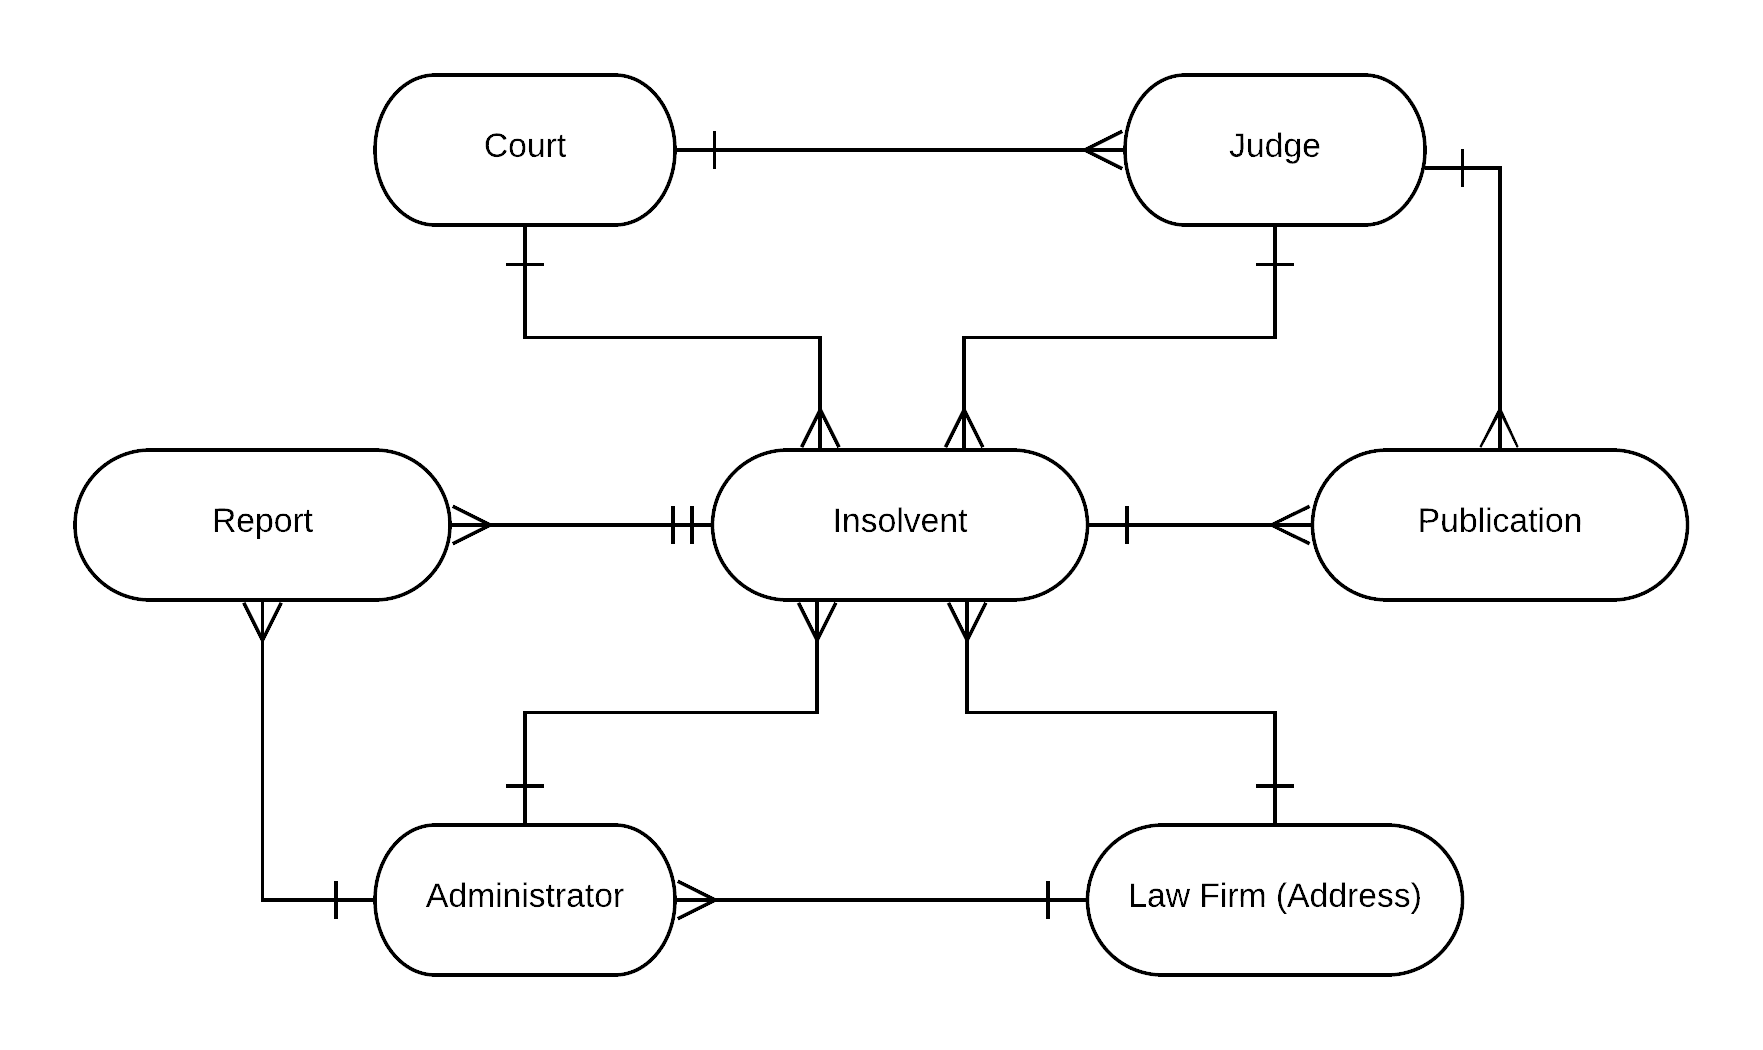
\includegraphics[width=1\linewidth]{cir_erd.png}
\caption{Insolvency entity relations.}
\end{figure}

The CIR XML data is structured: the entities are connected in the XML response by composition as defined in XSD schemas provided by CIR. Unique identifiers exist for the Insolvent, Publication and Report entities. An ETL (Extract Transform Load) component is build to load these entities into normalized SQL tables.

\paragraph{Database normalization}
Not all the data is normalized. The entities Judges and Administrators have no identifiers but consist of free text fields for their name (parts). This leads to unwanted duplication as names can be written in many different forms and typos can be introduced, e.g. one judge's name appears as:

\begin{itemize}
\item "mr. W.J. Geurts - de Veld"
\item "mr. W.J. Geurts-deVeld"
\item "mr. W.J. Geurts-de Veld"
\item "mr. W.J.Geurts-de Veld"
\item "mr.W.J. Geurts-de Veld"
\item "mr. W.J. Geurts-de Veld (Rotterdam)"
\item "mr W.J.Geurts-de Veld"
\item "W.J.Geurts-de Veld"
\end{itemize}

We need to define so-called master data for judges and administrators and resolve the duplicated names to the master data records. The two data sources in the sections \ref{NOvA Tableau} and \ref{Nevenfuncties Rechters} are chosen for this purpose.

\paragraph{PDF report web service}
A second web service operated by CIR provides Administrator Reports in PDF format using a simple HTTP GET request. There are two types of reports: 
\begin{enumerate}
\item progress reports
\item financial attachments
\end{enumerate}
Recofa has published templates for both report types\cite{rechtspraak:3}. The reports hold much of the unstructured data.

\subsubsection{Register of lawyers, NOvA Tableau}\label{NOvA Tableau}

The NOvA tableau is the official register for lawyers and maintained by the \textit{Nederlandse Orde van Advocaten (NOvA)}\cite{nova:1}. NOvA offers an on-line search form where key word search and filters can be applied to search for a lawyer. By looking at the network traffic we see than the form is powered by a REST API returning JSON data which we can employ directly. This data source is used to collect the master data for Administrators.

\subsubsection{Register of judges, Nevenfuncties Rechters}\label{Nevenfuncties Rechters}

The Register for ancillary positions for judges is made available by \textit{de Rechtspraak}\cite{rechtspraak:2}. It offers an on line form and returns the name, current and historical occupation and ancillary positions. Again, this form is powered by a REST API returning JSON which we can employ directly. This data source is used to collect the master data for Judges.


\subsection{Description of the system}
Figure \ref{System overview} gives an overview of the system components for extracting, enriching and integrating the sourced data and making the resulting structured and higher level information available to the user.

\begin{figure}[h]
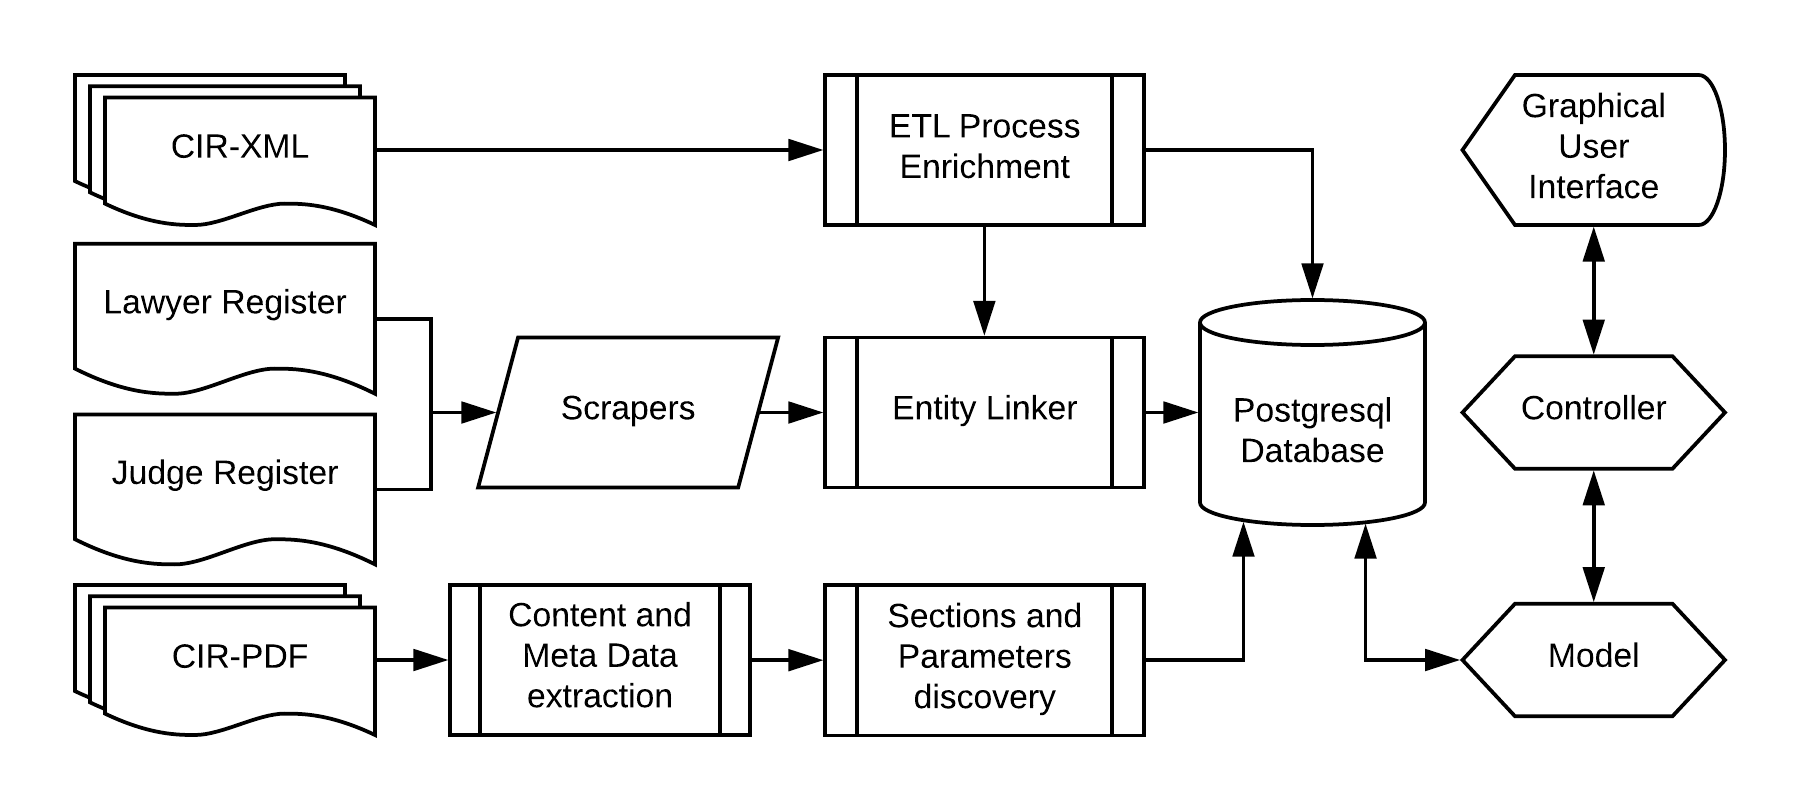
\includegraphics[width=1\linewidth]{system_overview.png}
\caption{System overview.}\label{System overview}
\end{figure}

\paragraph{The ETL process} This component extracts the entities and selected data fields from the XML. The data is enriched and annotated after which it is stored in the Postgresql database. An example of the enrichment are the start and end date of the insolvency which is not directly stated in the insolvency case XML.

\paragraph{The Entity Linker} This component is responsible for linking judges and administrators in CIR to real life entities found in the judge and lawyer registers. It does this by normalization of the CIR names and resolving them to the register entities using similarity functions. Unresolved entities are linked manually to establish complete linkage. Established links are stored in an association table. After an initial run the register scrapers are called upon only when new judge or administrator entries appear in CIR.

\paragraph{PDF processors}
PDF reports are processed to extract text content and meta data. In a subsequent process the text sections as defined in the progress report and key data parameter are discovered. These fields are available for search later on.

\paragraph{Model-View-Controller}
This is a well established pattern of three subcomponents working together. The user operates a graphical interface prototyped in Jupyter notebooks to query the data or interact with data visualisations or tables. This is the view in the MVC component. On user command, the controller asks the model to prepare the data and returns the data to the view.

